\chapter{Non-monotonic Reasoning in FCA}
\label{chapter:defeasible-reasoning-in-fca}

The conclusion of \Cref{part:1} marks the end of the scaffolding component of this work. The remaining
chapters are devoted to the introduction and subsequent discussion of the more novel contributions we make.
Namely, the unification of the ideas presented in
\Cref{chapter:formal-concept-analysis,chapter:defeasible-reasoning}. That is, to introduce an approach to do
the KLM style of non-monotonic reasoning in FCA. Fortunately, as will become apparent as this chapter
progresses, the setting of FCA may be quite naturally extended to accommodate the necessary semantics.

This chapter draws on two publications, \cite{Carr2024} and \cite{Carr2025}.

\section{Motivation}
\label{section:motivation}

We begin this unification by providing justification for why it may be desirable to extend FCA to support
non-monotonicity to begin with. There are certain properties of FCA that are substantially undermined by
violations of monotonicity. For instance, one central notion of concept lattices is that they describe chains
of inheritance between concepts and their sub-concepts. The ability to preserve these inheritance chains
becomes tenuous under non-monotonic semantics, as they are essentially a form of transitivity, which has
already been shown not to hold in KLM–style reasoning.

That being said, there are indeed compelling arguments that the presence of monotonicity in FCA has similarly
undesirable second-order effects. These are somewhat similar to those given in \Cref{section:nmr-background},
but phrased from a different perspective. The perspective change stems from the dissimilarity between the
starting point of the usual KLM setting and the starting point of FCA. In the former, one begins with a
knowledge base of implications, to which new rules are added. The addition of new information may result in
tension between deductions, which provides the motivation for defeasible reasoning. In contrast, the starting
point of FCA usually begins with a formal context, which is presumed to be static. One task is then to
perform a kind of rule learning of attribute implications, to discover corrpondence between attributes.

In the classical setting, only those attribute correspondences which are total, meaning they admit no counter
examples, can be found. To recognise that this implies monotonicity, suppose the rule $(\texttt{Beige}
	\rightarrow \texttt{Shade})$ were accpeted. Then every object which had the attribute \texttt{Beige} also has
\texttt{Shade}, by extension, every object that has \texttt{Beige} and \textit{something else} will continue
to have \texttt{Shade}. In certain cases, this imposes too strong an impediment on the amount of useful
information that may be extract from a context. Certainly, there are instances of meaningful correspondence
between attributes which admit exceptions. Herein lies the first motivation for introducing KLM style
reasoning to FCA. A second argument, consdering how the benefits of being able to reason prototypically about
concepts is presented in the next chapter, where it is more relevant.

Consider \Cref{cxt:lichens} below, which describes several distinct species of lichen, described by certain
morphological and ecological properties.

\begin{figure}[H]
	\hspace{-6.5em}
	\resizebox{1.1\textwidth}{!}{
		\centering
		\begin{cxt}
			\label{cxt:lichens}
			\cxtName{\textbf{\texttt{lichens}}}
			\atr{\texttt{Direct Light}}
			\atr{\texttt{Indirect Light}}
			\atr{\texttt{Shade}}
			\atr{\texttt{Heat}}
			\atr{\texttt{Dessication}}
			\atr{\texttt{Humidity}}
			\atr{\texttt{Cold}}
			\atr{\texttt{Bark}}
			\atr{\texttt{Rock}}
			\atr{\texttt{Soil}}
			\atr{\texttt{Debris}}
			\atr{\texttt{Moss}}
			\atr{\texttt{Leaf}}
			\atr{\texttt{Constructed}}
			\atr{\texttt{Thallus Crustose}}
			\atr{\texttt{Thallus Fruticose}}
			\atr{\texttt{Thallus Foloise}}
			\atr{\texttt{Thallus Byssoid}}
			\atr{\texttt{Orange}}
			\atr{\texttt{Yellow}}
			\atr{\texttt{Red}}
			\atr{\texttt{Pink}}
			\atr{\texttt{Bright green}}
			\atr{\texttt{Beige}}
			\atr{\texttt{Brown}}
			\atr{\texttt{Gray}}
			\atr{\texttt{Gray-white}}
			\atr{\texttt{Blue-gray}}
			\atr{\texttt{Blue-black}}
			\atr{\texttt{Gray-green}}

			\obj{.x.......x.................x.x}{\texttt{Caeruleum terricola}}
			\obj{x..xx.x.x.....x...x.x.........}{\texttt{Caloplaca marina}}
			\obj{x..xxxxxx....x..x.xx..........}{\texttt{Xanthoria parietina}}
			\obj{x..x.xx...x....x..xx..........}{\texttt{Teloschistes chrysophthalmus}}
			\obj{x..xx..xx.......x.....x.......}{\texttt{Crocodia aurata}}
			\obj{x..xx.x.x.......x...x....x....}{\texttt{Lasallia rubiginosa}}
			\obj{..x....xx.......x......xx..x.x}{\texttt{Sticta beauvoisii}}
			\obj{..xxx..xx...x..x.......x......}{\texttt{Ramalina celastri}}
			\obj{x..xx.x..x...xx...x.xx........}{\texttt{Psora crenata}}
			\obj{..x...x.xx......x.......x..x.x}{\texttt{Leptogium menziesii}}
			\obj{..xxxxx.xx.x....x.......x....x}{\texttt{Scytinium gelatinosum}}
			\obj{..x...x.xx.x..x...........x..x}{\texttt{Lepraria borealis}}
			\obj{.x.xx.xxxxxx..x...........xx.x}{\texttt{Lepraria caesiella}}
			\obj{..xx.xxx......x....x..........}{\texttt{Chrysothrix candelaris}}
			\obj{..x.......x......x.....x..x...}{\texttt{Roccellinastrum-lagarostrobi}}
			\obj{.x.xx.....x......x........x...}{\texttt{Roccellinastrum-spongoideum}}
			\obj{..x...xx...xx.x.........xx....}{\texttt{Thelenella-indica}}
			\obj{.x....x.x......x............x.}{\texttt{Usnea aurantiaco-atra}}
		\end{cxt}
	}

	\caption{A formal context of lichens} \label{fig:lichens}
\end{figure}

For no reason other than that it is interesting, some contextual information about lichen is provided.
\textit{Lichens} are not singular organisms, but rather a symbiosis between a fungus and alva
\cite{zonca2022lichens}. While they have previously been considered plants, lichens do not possess roots or
stalks. Instead, they are affixed to a particular substrate; tree-bark or moss, for instance. While in many
cases a lichen's substrate is itself a living organism, lichen are not parasitic. They derive no nutritional
value from their substrates and require them only for stability.

\subsection{Association Rules}
\label{subsection:association-rules}

Concerns over brittleness in the semantics of (classical) attribute implications are well known in the FCA
literature, and in data mining more generally \cite{Lakhal2005}. \textit{Association rules} are able express
implication-like statements despite the existence of counterexamples in the data, or in our case a context.
These are statements like \say{$66\%$ of the members of congress who were \textit{Democrats}, which makes up
	$50\%$ of congress, voted on the \textit{MX-Missile} bill}.

The \emph{support} of a set of attributes $X \subseteq M$ in a context $\GMI$ is the fraction of objects
which have all attributes $X$ over the total number of objects; and so $\mathrm{supp}( X) =
	\nicefrac{|X^{\downarrow}|}{|G|}$, the (relative) support of a rule $A \Rightarrow B$ is simply the support
of $A$. The \textit{confidence} of a rule is a measure of how frequently the premise and conclusion occur,
relative to how frequently the premise occurs, formally $\mathrm{conf}(A \Rightarrow B) =
	\nicefrac{\mathrm{supp}(X \cup Y)}{\mathrm{supp}(X)}$. In the example above, the support of the rule is
$50\%$ and its confidence is $66\%$. Association rules which meet specified lower-thresholds for support and
confidence are then accepted.

While association rules present a reasonable solution to the problem of discovering and representing
implications with exceptions, there are some undesirable qualities. Settling on the threshold vallues for
support and confidence is usually dependent on human input, and there is no obvious intuition for how one
might arrive at these. Frequently, it is a requirement to know the data well, which creates a kind of
circularity as the purpose of this work is to extend a tool which helps one understand their data.

The situation gets worse when we try to describe the properties of reasoning with association rules. Consider
the two rules below, which should be accepted with $\mathrm{minconf}= 0.6$ and $\mathrm{minsup}= 0.5$.

\begin{align*}
	\texttt{dem}\Rightarrow \texttt{mxm} \\
	% ; \text{with}\; \mathrm{Sup}= 0.5 \; \text{and}\; \mathrm{Conf}= 0.66 \\
	\texttt{dem}\Rightarrow \texttt{dfe} % \; \text{with}\; \mathrm{Sup}= 0.5 \; \text{and}\; \mathrm{Conf}= 0.66
\end{align*}
In natural language, we might summarise this scenario as saying \say{Democrats voted in favour of the
	\textit{MX-Missile} and \textit{Duty-Free Exports}}. To make future analysis simpler, we could suggest that
whenever we accept association rules of the form
\begin{align*}
	\phi \Rightarrow \psi \\
	\phi \Rightarrow \gamma,
\end{align*}
we may compress the information as the simpler representation:
\begin{align*}
	\phi \Rightarrow \psi \land \gamma
\end{align*}

Unfortunately, this is not always the case. In the above scenario, the rule $\texttt{dem}\Rightarrow
	\{\texttt{mxm,dfe}\}$ has a confidence of $0.47$, which is below the $\mathrm{minconf}$ threshold.

That the pattern of reasoning enforced by association rules does not satisfy the above
characterisation---which is the same property as was discussed at \Cref{postulate:and}---may be overlooked in
isolation. The more general problem is that association rules do not admit description via \lucas{the kind of
	axiomisation we want [source needed]}.

\section{Preferential Contexts}
\label{section:preferential-contexts}

We begin the introduction of KLM style defeasible reasoning to FCA by defining a structure that is in almost
perfect analogy to preferential interpretations. The analogy is not perfect as we initially behave quite
conservatively, and attempt to make as few changes to the default setting of FCA as possible. As we get
further along in this discussion, more substantial amendments to the default setting are suggested. These
will serve to complete the analogy. The idea behind the order of this exposition is that we view this work
largely as extending FCA with ideas borrowed from defeasible reasoning. Then, there may be those who find
some of the essential parts of defeasible reasoning quite useful in FCA, but wish to remain in the default
setting.

With that said, we define the first extension of a \textit{preferential context}.
\begin{definition}
	\label{definition:preferential-context}
	\index{formal context! preferential context}

	A \emph{preferential context} $\pcontext = \PGMI$ is a formal context $\GMI$ where $\prec$ is a strict
	partial order, or \emph{preference order}, on the set of objects.
\end{definition}

Preferential contexts, albeit with a different motivation, were first introduced by Obiedkov
\shortcite{Obiedkov2012} and later, with our purposes in mind, by Carr \textit{et al.} \shortcite{Carr2024}.
In some sense they are nothing more than a formal context with the addition of a preference order over the
set of objects. The same understanding of preference orders on states applies, and so for two objects $g_1,
	g_2 \in G$, when $g_1 \prec g_2$, we say that object $g_1$ is \textit{preferred} or \textit{more typical}
than $g_2$.

Much like the case of preferential interpretations in propositional logic, it is required that the preference
relation be well-founded. Of course, any preferential context where the set of objects is finite will be
well-founded. %TODO what happens with infinite attribute sets

An example of what such a preference ordering might look like is given below (in the interests of brevity, we
consider only a subcontext of \Cref{cxt:lichens}, constructed by taking the first six objects).

\begin{figure}[H]
	\centering
	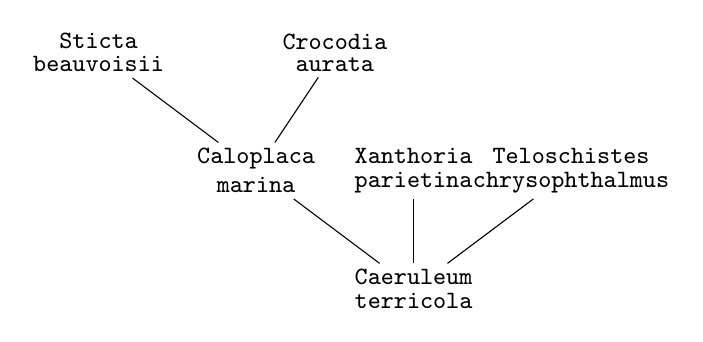
\begin{tikzpicture}[every node/.style={text=black, inner sep=2pt, font=\small}]
		\node (root) at (0,0) {\shortstack{\texttt{Caeruleum}\\\texttt{terricola}}};
		\node (1) at (-2,1.5) {\shortstack{\texttt{Caloplaca}\\\texttt{marina}}};
		\draw (root) -- (1);
		\node (2) at (0,1.5) {\shortstack{\texttt{Xanthoria}\\\texttt{parietina}}};
		\draw (root) -- (2);
		\node (3) at (2,1.5) {\shortstack{\texttt{Teloschistes}\\\texttt{chrysophthalmus}}};
		\draw (root) -- (3);
		\node (12) at (-4,3) {\shortstack{\texttt{Sticta}\\\texttt{beauvoisii}}};
		\draw (1) -- (12);
		\node (13) at (-1,3) {\shortstack{\texttt{Crocodia}\\\texttt{aurata}}};
		\draw (1) -- (13);
	\end{tikzpicture}
	\caption{A preference relation on a subcontext of \Cref{fig:lichens}}
	\label{figure:preference-relation-lichen}
\end{figure}

Recall that preferential interpretations were defined by a relation on states, which were subsequently mapped
to valuations, with no requirement that the mapping be injective. That is, the same valuation could appear in
multiple ``locations'' in the preference order. It may then be surprising that states see have been entirely
omitted from our definition of preferential contexts. The reason is slightly informal and based on the
recognition that, unlike the set of propositional valuations, formal contexts have no restriction on the
inclusion of distinct objects with equivalent intensions. In fact, this is quite common. If need be, one may
quite naturally avoid the issue arising from duplicate states introduced in \Cref{lemma:states-preferential}.

% \begin{lemma}
% 	\label{lemma:objects-preferential}
%
% 	There exists a preferential context $\pcontext = \PGMI$ where there exist two objects, $g,h \in G$, with
% 	$g^{\uparrow}= h^{\uparrow}$ that defines the consequence relation $\twiddle_{\pin}$ such that no
% 	preferential context $\pcontext'$ without `duplicate' objects defines the same relation.
% \end{lemma}

Under the preference relation, we describe the $\prec$-minimal states as one might expect, through the
process of \textit{minimisation}.

\begin{definition}
	\label{definition:minimisation}

	In a preferential context $\pcontext = \PGMI$, the \emph{minimisation} of a set $A \subseteq G$ is defined by
	\[
		\underline{A}\coloneqq \{\, g \in A \mid \nexists h \in A : (h \prec g) \,\}.
	\]
\end{definition}

Frequently, the starting point of a minimisation is not directly from a set of objects, and is rather applied
to a set of objects that is itself the result of a prior derivation of attributes. That is, we might begin
with the attribute set $\{\,\texttt{soil}\,\}$ and wish to find the most preferred objects that have this
attribute. We call this the \textit{minimised-derivation}, and write $\Mind{\{\,\texttt{soil}\,\}}$. If one
were to apply a second derivation to the set resulting from a minimised-derivation, the result would
represent all those attributes shared by the preferred objects that were in the minimised-derivation from the
initial set of attributes. In turn, we refer to this as \textit{minimised-return} and write
$\Minr{\{\,\texttt{soil}\,\}}$.

The minimised-derivation of $\{\,\texttt{soil}\,\}$ yields the singleton object-set \{\texttt{Caeruleum
	terricola}\}. One interpretation of this might be that the lichen species, \texttt{Caeruleum terricola}, has
some soil-substrate related property which sets it apart from other species of lichen which also possess a
soil-substrate. The point is subtle, but this interpretation of what the preference order conveys is not true
in general. The status of \texttt{Caeruleum terricola} as the uniquely preferred species of lichens which
have a soil-substrate may well be the byproduct of another preference, entirely unrelated to substrates. For
example, \Cref{figure:preference-relation-lichen} may be an encoding of the preference that \say{lichens
	which tolerate indirect light are more preferable than those which tolerate direct light; from those
	less-preferrable species which do tolerate direct light, it is preferred that they are orange}. These
preferences would construct the same ordering on objects, but clearly has a distinct interpretation to that
which was proposed previously. This remark is of little material significance, but is rather important for
preventing misconceptions about what preference orders represent, and provides some intuition for how they
might be constructed. For the time being, we remain agnostic to the latter question about their construct.
This will be the subject of \Cref{subsubsection:finding-order}.

Our motivation for introducing preferential contexts is quite apparent: their structural properties can be
used to provide a semantics for defeasible attribute implications, which we refer to as \textit{defeasible
	conditionals}.

\begin{definition}
	\label{definition:satisfaction-preferential-context}

	Let $\pcontext = \PGMI$ be a preferential context, $A,B \subseteq M$ subsets of attributes, and $A \twiddle
		B$ \emph{defeasible conditional}. We say that $A \twiddle B$ is \emph{satisfied} by $\pcontext$ if and only
	if $\Mind{A}\subseteq B^{\downarrow}$, then we write $\pcontext \vDash_{\pcontext}A \twiddle B$.
\end{definition}

Fortunately, the definition of what it means for a defeasible conditional to be satisfied by a preferential
context is very similar to what it means for a attribute implication to be satisfied by a regular context.
Indeed, so similar that it is quite trivial to recognise that defeasible conditionals are supraclassical. If
a classical implication $X \rightarrow Y$ holds in a context, then $X^\downarrow \subseteq Y^\downarrow$. The
minimised-derivation of $X$ is always a subset, and so the condition follows immediately. In the, more
common, case where we consider non-classical implications, the intended meaning of $X \twiddle Y$ is that all
those most preferred objects in the extension of $X$ are also included in the extension of $Y$. If the
conditional holds in a preferential context, it is also equivalent to the familiar expression that $Y
	\subseteq \Minr{X}$.

\begin{example}

	For an illustration, consider the preferential context that is composed from \Cref{cxt:lichens} and the
	preference order described in \Cref{figure:preference-relation-lichen}.

	\begin{figure}[H]
		\hspace{-6.5em}
		\resizebox{1.1\textwidth}{!}{
			\centering
			\begin{cxt}
				\label{cxt:lichens-small}
				\cxtName{\textbf{\texttt{lichens}}}
				\atr{\texttt{Direct Light}}
				\atr{\texttt{Indirect Light}}
				\atr{\texttt{Shade}}
				\atr{\texttt{Heat}}
				\atr{\texttt{Dessication}}
				\atr{\texttt{Humidity}}
				\atr{\texttt{Cold}}
				\atr{\texttt{Bark}}
				\atr{\texttt{Rock}}
				\atr{\texttt{Soil}}
				\atr{\texttt{Debris}}
				\atr{\texttt{Constructed}}
				\atr{\texttt{Thallus Crustose}}
				\atr{\texttt{Thallus Fruticose}}
				\atr{\texttt{Thallus Foloise}}
				\atr{\texttt{Thallus Byssoid}}
				\atr{\texttt{Orange}}
				\atr{\texttt{Yellow}}
				\atr{\texttt{Red}}
				\atr{\texttt{Bright green}}

				\obj{.x.......x..........}{\texttt{Caeruleum terricola}}
				\obj{x..xx.x.x...x...x.x.}{\texttt{Caloplaca
						marina}}
				\obj{x..xxxxxx..x..x.xx..}{\texttt{Xanthoria parietina}}
				\obj{x..x.xx...x..x..xx..}{\texttt{Teloschistes chrysophthalmus}}
				\obj{x..xx..xx.....x....x}{\texttt{Crocodia
						aurata}}
				\obj{x..xx.x.x.....x...x.}{\texttt{Lasallia rubiginosa}}
				\obj{..x....xx.....x.....}{\texttt{Sticta
						beauvoisii}}
			\end{cxt}
		}
	\end{figure}

	Example shoudl talk about how we are fitting a rule-set to data, unlike the original KLM setting. Somewhat
	similar to inductive-logic-prgoramming
	% The following defeasible conditionals are all satisfied by the preferential
	% context composed from \Cref{cxt:lichens} with the preference order from
	% \Cref{figure:preference-relation-lichen}.
	%
	% \begin{enumerate}[nosep]
	% 	\item $\{\texttt{high-light}\} \twiddle \{\texttt{red}\}$
	% 	\item $\{\texttt{high-light,low-moisture}\} \ntwiddle \{\texttt{red}\}$
	% 	\item $\{\texttt{high-light, yellow}\} \twiddle \{\texttt{orange}\}$
	% 	\item $\{\texttt{orange}\} \twiddle \{\texttt{red}\}$
	% 	\item $\{\texttt{high-light,yellow}\} \ntwiddle \{\texttt{red}\}$
	% \end{enumerate}
	%
	% These conditionals convey that usually species of lichen that live in areas
	% with a signficant amount of light are red, but those which additionally live in
	% areas with low-moisture usually are not red. While it is typical for yellow
	% species of lichen that live in well-lit areas to also be orange, and it is also
	% typical for orange species of lichen to have red colouring too, it does not
	% follow that yellow species of lichen living in well-lit areas have red. In
	% other words, the logic is non-monotonic and intransitive.
\end{example}

If not for the warnings at the start of this section, it might be suspected that the kind of reasoning
described by preferential contexts corresponds to the preferential consequence relations discussed earlier.
We show that this is not quite true.

\begin{theorem}
	\label{theorem:preferential-context-partial-soundness}

	The consequence relation $\twiddle_{\pcontext}$ induced by a preferential context $\PGMI$ satisfies
	\textit{Reflexivity, Left-logical equivalence, Right weakening, And,} and \textit{Cautious Monotony}.
\end{theorem}

\begin{proof}
	\label{proof:preferential-context-partial-soundness}

	Let $\pcontext = \PGMI$ be a preferential context, and $A,B,C,D \subseteq M$ sets of attributes.

	For \textit{Reflexivity}, it needs to be shown that $\pcontext \vDash A \twiddle A$, equivalently that
	$\Mind{A}\subseteq A^{\downarrow}$. This holds by definition of the minimal-derivation operator. \lucas{Make
		sure this holds if $A^{\downarrow}= \emptyset$}

	For \textit{Left-logical equivalence}, if $\pcontext \vDash_{\pcontext}A \twiddle C$ and $A = B$, then
	$\pcontext \vDash_{\pcontext}B \twiddle C$. Assume that $\pcontext \vDash A \twiddle C$ and $A = B$ (by usual
	set equality). By this assumption, (i) $\Mind{A}\subseteq C^{\downarrow}$ and (ii) $\Mind{A}= \Mind{B}$ both
	hold. It is then clear that we can make the substitution that results in $\Mind{B}\subseteq C^{\downarrow}$,
	which is equivalent to $\pcontext \vDash B \twiddle C$.

	For \textit{Right weakening} we show that if $\pcontext \vDash A \rightarrow B, B \twiddle C$ then $\pcontext
		\vDash A \twiddle C$.
\end{proof}

The failure to satisfy the \textit{Or} postulate is due more to a technical point, rather than the existence
of any particular counter example. The assumed setting of FCA's attribute logic is restricted to definite
Horn clauses, and therefore not sufficiently expressive for either negation or disjunction. With these
notions absent from the language, we may not fulfill the missing postulate. However, preferential contexts
and the corresponding semantics for defeasible conditionals correspond to \textit{cumulative consequence
	relations} \cite{kraus1990nonmonotonic}, the weakest of the systems in the KLM framework. Discussion of
cumulative consequence relations was omitted from \Cref{chapter:defeasible-reasoning} as they are subsumed by
preferential consequence relations, without much interesting distinction.

This issue may be addressed by considering a more expressive variant of attribute logic: the logic of
compound attributes discussed in \Cref{subsection:compound-attributes}. Given that compound attributes are
built on top of a set of ``normal'' attributes, the original definition of a preferential context is
sufficient. It is only necessary to change the language of defeasible conditionals.

\begin{definition}
	\label{definition:defeasible-conditionals-compound}

	Let $\pcontext = \PGMI$ be a preferential context. Then $\phi \twiddle \psi$ where $\phi,\psi \in M^{+}$ is a
	\emph{defeasible conditional} over the compound attributes of $M$.
\end{definition}

We re-emphasize the point, which was originally made in \Cref{section:klm-framework}, that although the
formulae that make up the antecedent and consequent of a defeasible conditional $\phi \twiddle \psi$ are in
the language $M^{+}$, they are not themselves allowed to be defeasible conditionals. Thus, nesting of
defeasible conditionals---resulting in expressions such as $\phi \twiddle \gamma \twiddle \psi$---is not
permitted. Fortunately, with the relatively minor extension of compound attributes, the logic is sufficiently
expressive for disjunction, and so we construct the following representation result.

\begin{theorem}
	\label{theorem:preferential-context-soundness}

	The consequence relation $\twiddle_{\pcontext}$ induced by a preferential context $\pcontext = \PGMI$ with
	defeasible conditionals over the compound attributes of $M$ is a preferential consequence relation.
\end{theorem}

% \begin{proof}
% 	\label{proof:preferential-context-soundness}
% \end{proof}

% \begin{theorem}
% 	\label{theorem:preferential-context-completeness}

% 	Let $\twiddle_{P}$ be an arbitrary preferential consequence relation over compound attributes $M^{+}$. Then
% 	there exists a preferential context $\pcontext = \PGMI$ inducing the consequence relation
% 	$\twiddle_{\pcontext}$ such that $\twiddle_{P}$ is precisely $\twiddle_{\pcontext}$.
% \end{theorem}

% \begin{proof}

% 	\label{proof:preferential-context-completeness}
% \end{proof}

% \begin{proposition}
% 	\label{proposition:preferential-context-irrational}

% 	Preferential contexts do not satisfy rational monotony.
% \end{proposition}

% % \begin{example} \label{example:counter-example-rationality} \end{example}

% \begin{definition}
% 	\label{definition:ranked-context}

% 	A \emph{ranked context} $\rcontext$ is a preferential context $\RGMI$ where the preference relation
% 	$\mathsf{R}$ on objects is a \textit{strict weak order}.
% \end{definition}

\subsubsection{Finding Order}
\label{subsubsection:finding-order}

% Thus far, the discussion on finding a suitable preference relation has been omitted. It is a non-trivial task
% to compare objects in a context.

\begin{algo}{\textsc{ObjectRank}}
	\label{algorithm:ObjectRank}

	\Require A set $\Delta$ of defeasible conditionals over an attribute set $M$
	\Require A formal context $\GMI$
	\Ensure A ranking $\mathsf{R}\colon G \to \mathbb{N}$ such that $\Delta$ holds in $\RGMI$ if $\GMI$ is $\Delta$-compatible; $\bot$, otherwise.
	\State $i \coloneq 0$
	\State \textit{initialise} $\mathsf{R}(g) \coloneq \vert G \vert$ for all $g \in G$
	\State $\Gamma \coloneq \Delta$
	\While{$\exists \, g \in G \colon \mathsf{R}(g) = \vert G \vert$}
	\ForAll{$g \in G$ with $\mathsf{R}(g) = \vert G \vert$}
	\If{$g \vDash \Gamma$}
	\State \textit{update} $\mathsf{R}(g) = i$
	\EndIf
	\If{$\forall \, g \in G \colon \mathsf{R}(g) \neq i$}
	\State \Return $\bot$
	\EndIf
	\State $\Gamma \coloneq \{(\phi \twiddle \psi) \in \Gamma \mid g \nvDash \phi \; \text{for all}\; g \in G
		\; \text{with}\; \mathsf{R}(g) = i\}$ \State $i \coloneq i + 1$
	\EndFor
	\EndWhile
	\State \Return $\mathsf{R}$
\end{algo}

% \section{Entailment}
% \subsection{Contextual Rational Closure}

% \begin{definition}

% 	A conditional $A \twiddle B$ \emph{rationally follows} from a set $\mathcal{T}$ of conditionals if and only
% 	if $\mathbb{T}, \mathcal{T}\dentails A \twiddle B$, where $\mathbb{T}$ is the \emph{test context}. It
% 	\emph{contextually follows} when $\mathbb{R}, \mathcal{T}\dentails A \rightarrow B$.
% \end{definition}

% \begin{definition}

% 	A set $\mathcal{T}$ is \emph{closed} with respect to a pair if and only if it contains every conditional that
% 	is rationally entailed. That is, if $\mathcal{T}= \{A \twiddle B \mid A,B \subseteq M \tand
% 		\mathbb{T},\mathcal{T}\dentails A \twiddle B\}$. $\mathcal{T}$ is \emph{contextually closed} if it contains
% 	every conditional that is contextually entailed, i.e. $\mathcal{T}= \{A \twiddle B \mid A,B \subseteq M \tand
% 		\mathbb{R}, \mathcal{T}\dentails A \rightarrow B\}$.
% \end{definition}

% \begin{definition}

% 	A set $\mathcal{T}$ of conditionals is \emph{rationally complete} with respect to $\mathbb{T},\Delta$ if and
% 	only if every conditional that is in the rational closure of $\mathbb{T}, \Delta$ rationally follows from
% 	$\mathcal{T}$, i.e., $\mathbb{T},\mathcal{T}$ and $\mathbb{T}, \Delta$ define the same entailment relation.
% \end{definition}
% Is it possible to find a$\mathcal{T}$such that$\mathcal{T}$is a compact form of$\Delta$. I.e., it should
% produce the same ranking on$\mathbb{T}$.

% \begin{definition}

% 	A set $\mathcal{T}$ of conditionals is \emph{contextually complete} with respect to $\mathbb{R}, \Delta$ if
% 	and only if every implication that is in the contextual closure of $\mathbb{R}, \Delta$ rationally follows
% 	from $\mathcal{T}$.
% \end{definition}

% A set of conditionals that is contextually complete to a ranked context$\mathbb{R}$and constraint
% set$\Delta$provides abstracted perspective, in terms of defeasible conditionals, on the information contained
% in the pair$(\mathbb{R}, \Delta )$. It is now the goal, as was done in
% \Cref{subsubsection:implication-bases}, to find such a set that is non-redundant, or the \textit{rational
% 	basis}of$(\mathbb{R},\Delta)$.

% \begin{definition}
% 	\label{definition:defeasible-closure}

% 	Let $\mathcal{T}$ be a set of defeasible conditionals over $M$. The operator $X \mapsto \Cn{\twiddle}(X)$
% 	given by $X \cup \{Y \subseteq M \mid X \twiddle Y\}$ is called the \emph{defeasible closure} of $X$. It is
% 	idempotent, extensive, and non-monotonic.
% \end{definition}

% \subsection{Rational Closure}

% \subsection{A Basis for Ranked Contexts}

% \subsection{Lexicographic Closure}

